\chapter{Herramientas y plataforma de desarrollo}
\label{cap:capitulo3}

El desarrollo de nuevo contenido para la plataforma de VisualCircuit, ha necesitado usar distintas herramientas, como por ejemplo middleware,
ROS2, simulador robótico Gazebo..., por lo que se va a hacer una pequeña descripción de cada una, así como el uso que se le ha dado dentro del proyecto.

\section{Lenguaje de programación Python}
\label{sec:lenguaje_programación_python}
% ** LENGUAJES DE PROGRAMACÍON
% ** PYTHON

Python\footnote{\textbf{Python ORG}: \url{https://www.python.org/}} es un lenguaje interpretado de alto nivel. Este lenguaje busca facilitar la legibilidad del código, convirtiéndolo en uno de los más comunes a día de hoy.
Es un lenguaje de programación multiparadigma, ya que soporta tanto programación orientada a objetos, como programación imperativa y funcional.\\

Python cuenta con un gran número de bibliotecas y módulos que se usarán a lo largo de las distintas prácticas realizadas, como la librería \textit{math} que
permite usar operaciones matemáticas complejas (senos, cosenos, generación de números pseudo-aleatorios...).

Este lenguaje de programación cuenta con varias versiones. La que se usará durante el TFG será python 3.8, ya que la programación dentro
de la plataforma VisualCircuit (\ref{sec:visualcircuit}) se hace en este lenguaje.

\section{ROS2 (Robot Operating System 2)}
\label{sec:ros2}
% ** MIDDLEWARE ROS2

ROS\footnote{\textbf{ROS}: \url{http://wiki.ros.org/es}} o Robot Operating System es un
\textit{middleware}\footnote{{\textbf{Middleware}: software que se sitúa entre las aplicaciones y el sistema operativo}} formado
por un conjunto de herramientas y librerías de software libre empleadas para el desarrollo de aplicaciones robóticas.
Su objetivo es ofrecer una plataforma de programación estándar para todas las ramas de la robótica.\\

ROS se basa en una arquitectura \textit{cliente-servidor} centralizado que, mediante suscriptores y publicadores, permite enviar información,
ya sean medidas de sensores, cambios de estado, decisiones usando árboles de decisión, órdenes a los actuadores, etc.\\

Para comunicarse con los servidores (o como se llaman en ROS, \textit{topics}) se usan nodos. Estos nodos pueden contar con varios publicadores y suscriptores
simultáneaos.
Cada \textit{topic} se define con un tipo de mensaje, que será el único que se pueda enviar y recibir a través de él. Estos tipos de mensajes pueden ser
mensajes simples como una cadena de caracteres o tipos compuestos con otros tipos, permitiéndonos crear topics adecuados a las necesidades de cada proyecto.

\begin{figure} [H]
    \begin{center}
        \includegraphics[width=6cm]{figs/c3/ros_comunicación.png}
    \end{center}
    \caption[Comunicación entre nodos ROS.]{Comunicación del nodo Master con los nodos Intermedios y con distintos sensores y actuadores. Imagen obtenida de \cite{comunicacion_ros2}}
    \label{fig:ros_master_comunicacion}
\end{figure}
ROS cuenta con dos versiones principales, ROS y ROS2\footnote{\textbf{Versiones de ROS}: \url{https://docs.ros.org/}}. ROS está pensado para usarse
únicamente en sistemas Ubuntu, mientras que ROS2 también se puede usar en OS X y Windows. En cuanto a lenguajes de programación, ROS usa C++03 y
python2 (aunque se puede cambiar reduciendo su optimización), frente a los lenguajes de ROS2 que permite usar tanto C++11, C++14 y python3.5 (versión mínima).
Dentro de ambas versiones hay distintas distribuciones, como por ejemplo ROS Kinetic, Melodic o Noetic, o ROS2 Foxy, Galactic o Humble.

A lo largo del proyecto se usará ROS2 Humble para obtener información del robot TurtleBot2 (\ref{sec:turtlebot2}), tanto real como simulado,
como por ejemplo su posición en el entorno simulado o las últimas medidas de sus sensores, y para comandarle instrucciones (velocidades a sus motores).

\subsection{Visualizador RVIZ2}
\label{subsec:rviz2}
% ** RVIZ2

ROS2\footnote{\textbf{RVIZ2}: \url{https://github.com/ros2/rviz/tree/humble}} cuenta con su propio depurador pensada para funcionar con topics.
Esta herramienta es RVIZ2, una herramienta de visualización 3D que nos permite interpretar gráficamente las medidas de los sensores,
así como la información de otros topics (ubicación del robot o de otros objetos, mapas 2D y 3D...).

\begin{figure} [H]
    \begin{center}
        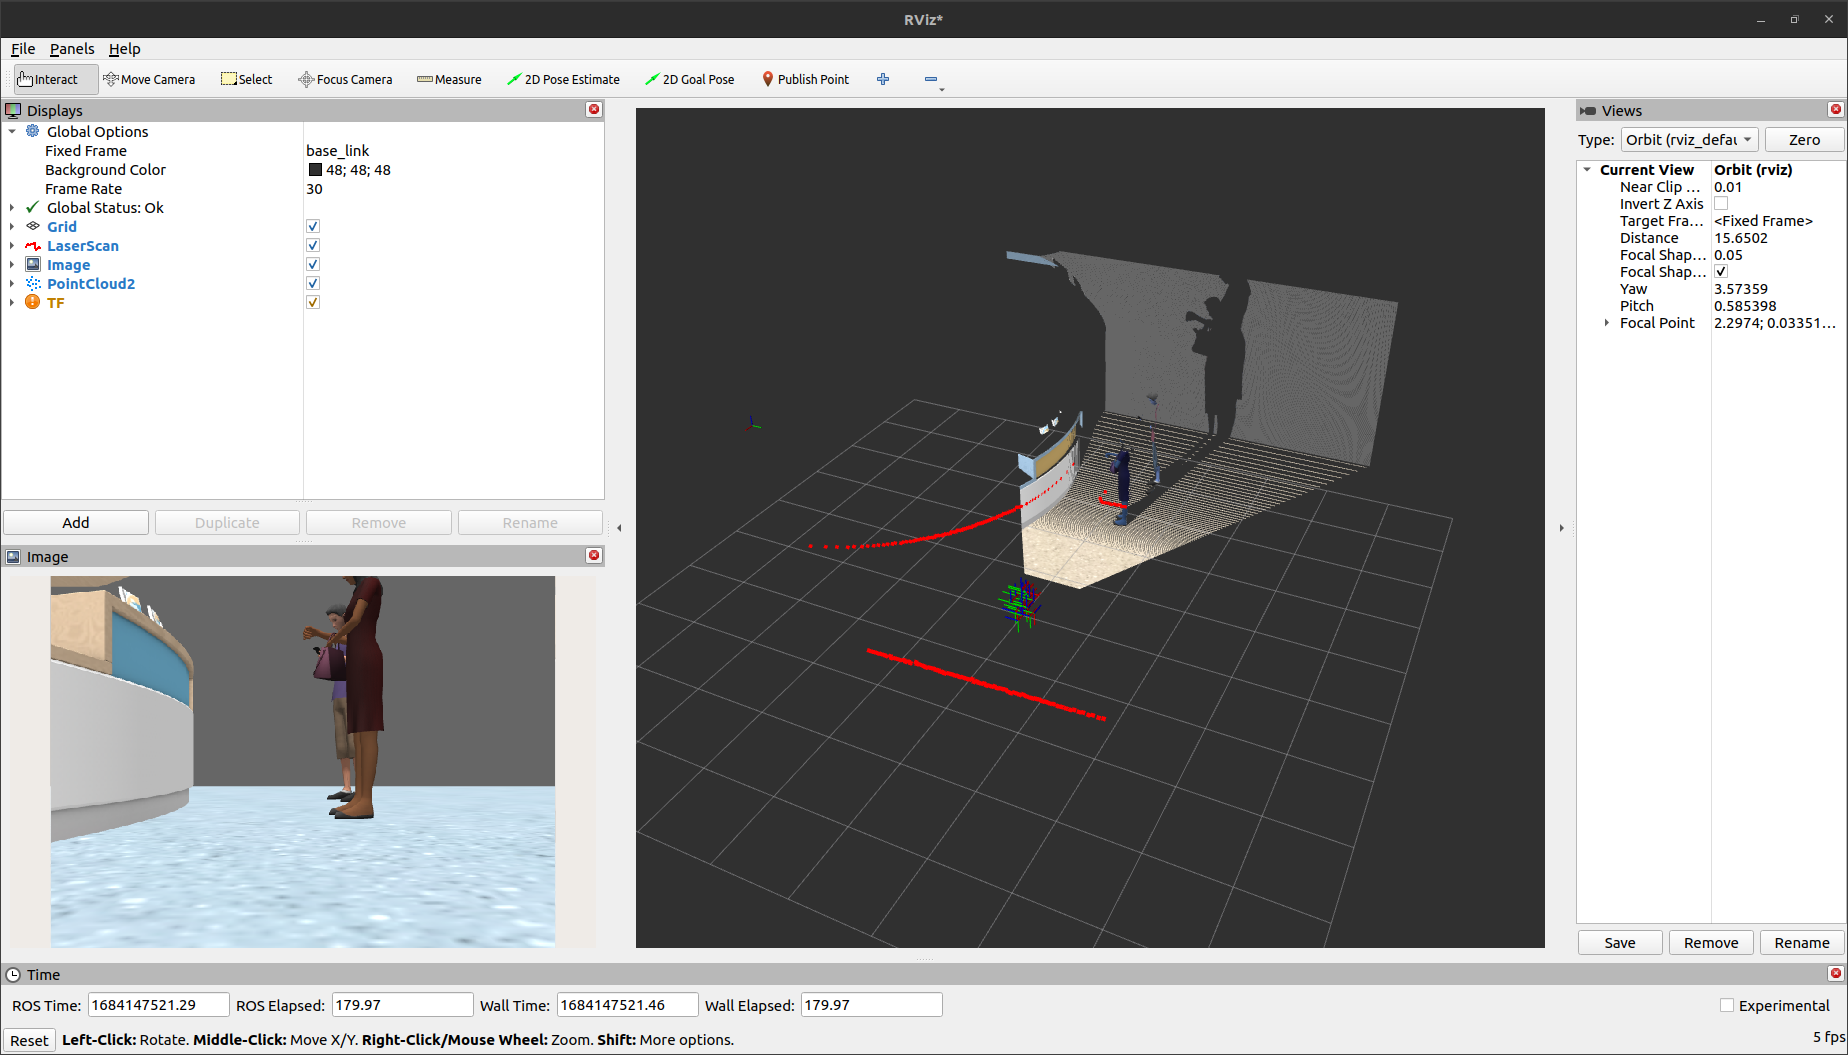
\includegraphics[width=12cm]{figs/c3/RVIZ2.png}
        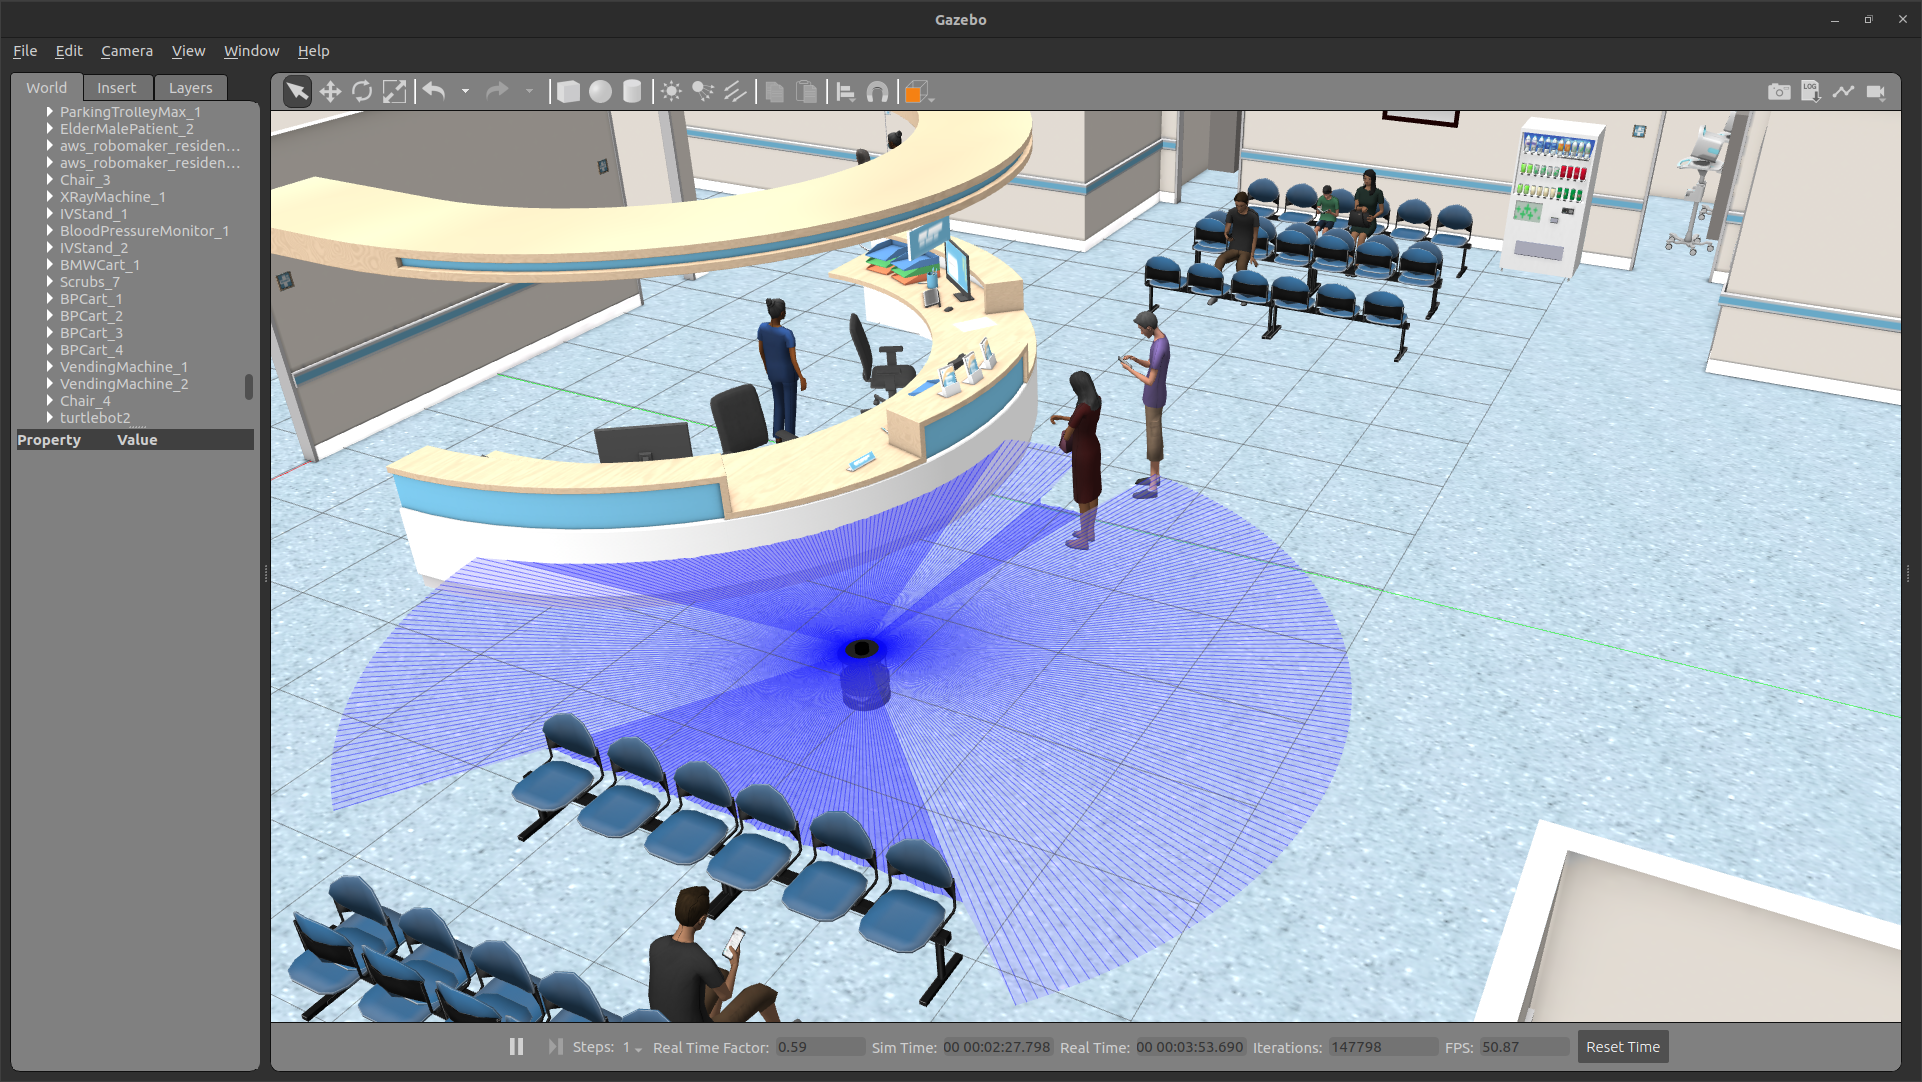
\includegraphics[width=12cm]{figs/c3/Gazebo_RVIZ.png}
    \end{center}
    \caption[RVIZ2 Vs mundo gazebo]{Ejemplo de RVIZ2 frente al mundo gazebo.}
    \label{fig:rviz2_example}
\end{figure}

\newpage

\section{TurtleBot2}
\label{sec:turtlebot2}
% ** TURTLEBOT2

La URJC de Fuenlabrada, en sus laboratorios de robótica, cuenta con varios robots 
TurtleBot2\footnote{\textbf{TurtleBot2}: \url{https://www.turtlebot.com/turtlebot2/}} a disposición de los alumnos del grado. Estos son perfectos para
la enseñanza e investigación en robótica, por su sencilla introducción a temas como ROS o el uso de sensores. Los TurtleBot2 están formados por dos partes
principales: una base Kobuki y una estructura superior.


\subsection{Base Kobuki}
\label{subsec:turtlebot2_base}
% ** TURTLEBOT2 -> KOBUKI

La base del TurtleBot2 se llama \textit{Kobuki}. En apariencia, es similar a un robot de limpieza como podrían ser los Roomba. En cuanto al hardware,
lleva integrados tres bumpers (sensores de contacto), odometría, sensor de caída y varios giroscopios. Tiene una velocidad lineal máxima de 0.7 m/s y
angular de 180 grados/s. Su batería le permite una autonomía de entre 3 y 7 horas. Cuenta con varios puertos, entre ellos un USB para poder conectar nuestro
portatil y ejecutar los distintos algoritmos.\\

Algunos de los paquetes de ROS2 que instalaremos para poder usarlo son los drivers del kobuki para
ROS2-Humble\footnote{\textbf{Drivers kobuki ROS2-Humble}: \url{https://github.com/IntelligentRoboticsLabs/Robots/tree/humble/kobuki}} de IntelligentRoboticsLabs,
compañeros de la URJC. Siguiendo las instrucciones de instalación que se encuentran en dicho repositorio de github, accedemos a varios paquetes básicos
para el uso de kobuki, como \textit{kobuki\_ros} o \textit{kobuki\_node}, entre otros.

\begin{figure} [H]
    \begin{center}
        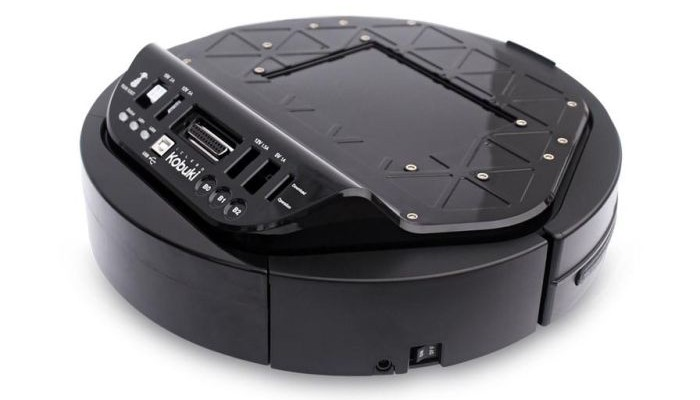
\includegraphics[width=7cm]{figs/c3/kobuki_base.jpg}
    \end{center}
    \caption[Kobuki base]{Base kobuki. Imagen obtenida de \cite{kobuki_base}}
    \label{fig:kobuki_base}
\end{figure}

\newpage

\subsection{Cuerpo Turtlebot2}
\label{subsec:turtlebot2_body}
% ** TURTLEBOT2 -> CUERPO
El cuerpo del TurtleBot2 (también conocido como \textit{TurtleBot Structure}) está formado por una serie de plataformas y tubos que se atornillan a la
base kobuki y permiten fijar nuevos sensores, como podrían ser una cámara o un láser, o actuadores como brazos robóticos. También ofrece un sitio cómodo
para poder colocar el portátil encima del robot y así poder conectarlo a la base mediante USB. 


\begin{figure} [H]
    \begin{center}
        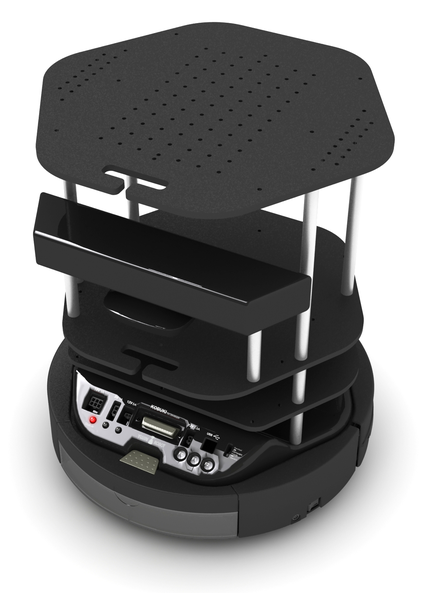
\includegraphics[width=5cm]{figs/c3/turtlebot2_body.jpg}
    \end{center}
    \caption[TurtleBot2]{TurtleBot2. Imagen obtenida de \cite{turtlebot_2_structure}}
    \label{fig:turtlebot_2_structure}
\end{figure}

\subsection{Cámara ASUS Xtion Pro}
\label{subsec:asus_xtion}
% ** ASUS XTION
La cámara \textit{ASUS Xtion} es una cámara RGB-D\footnote{\textbf{RGB-D}: RedGreenBlue-Depth, hace referencia las cámaras que captan la imagen y
las distancias de cada pixel.}, que ofrece tanto imagen como una nube de puntos con la distancia medida para cada pixel de la imagen.
Esta cámara ofrece una imágen de 720p, con una frecuencia de 60fps. En la parte de profundidad, es capaz de captar desde 0.8m hasya 3.5 con un
ángulo efectivo de 70º. Se conecta mediante USB directamente al ordenador.\\
En el proyecto, como debemos usarla con ROS2, usaremos el paquete creado por un usuario de
internet\footnote{\textbf{Drivers ASUS-Xtion ROS2}: \url{https://github.com/mgonzs13/ros2_asus_xtion}}.\\
\begin{figure} [H]
    \begin{center}
        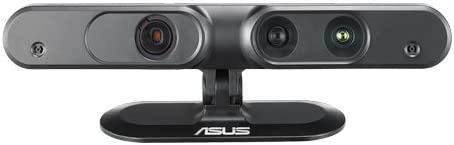
\includegraphics[width=5cm]{figs/c3/asus_xtion.jpg}
    \end{center}
    \caption[Cámara ASUS-XTION]{Cámara ASUS-XTION. Imagen obtenida de \cite{asus_xtion}}
    \label{fig:asus_xtion}
\end{figure}

\subsection{RPLIDAR A2}
\label{subsec:rplidar_a2}
% ** RPLIDAR

Se trata de un láser de 360º con un rango de medida desde 0.2m hasta 16m y una frecuencia de muestreo que se puede ajustar desde 5Hz hasta 15Hz.
Usando los drivers mencionados en el apartado del TurtleBot2 (\ref{subsec:turtlebot2_base}) encontraremos un paquete para poder activar y usar este sensor con ROS2.\\

\begin{figure} [H]
    \begin{center}
        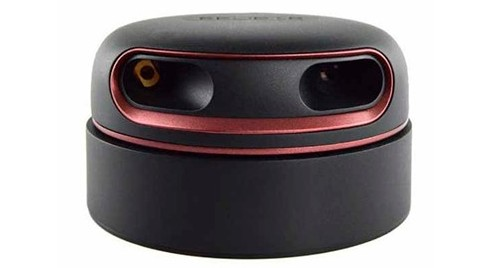
\includegraphics[width=5cm]{figs/c3/rplidar-a2.jpg}
    \end{center}
    \caption[RPLIDAR A2]{Sensor RPLIDAR A2. Imagen obtenida de \cite{rplidar}}
    \label{fig:rplidar}
\end{figure}

\section{Simulador robótico Gazebo}
\label{sec:gazebo}
% ** GAZEBO

\textit{Gazebo}\footnote{\textbf{Gazebo}: \url{https://classic.gazebosim.org/}} es un simulador 3D de código abierto orientado a la robótica que permite
fusionar escenarios realistas con robots simulados, ofreciendo un entorno seguro para probar algoritmos. Éste utiliza el motor de físicas
ODE\footnote{\textbf{Open Dynamics Engine}: \url{https://www.ode.org/}}, aunque se puede configurar con otros motores, como
Bullet\footnote{\textbf{Bullet}: \url{https://pybullet.org/wordpress/}} o DART\footnote{\textbf{DART}: \url{https://dartsim.github.io/}}.\\

Al estar orientado a la robótica, permite integrar fácilmente modelos de robots reales con sensores (incluso simulando sus ruidos) y enviar a través
de los distintos topics de ROS o ROS2 (\ref{sec:ros2}) alguna información directa del simulador, como la posición, medidas de los sensores simulados o
incluso información de objetos no programables (del entorno).\\

Actualmente Gazebo cuenta con dos versiones principales, \textit{Gazebo classic}\footnote{\textbf{Gazebo classic}: \url{https://classic.gazebosim.org/}} e
\textit{ignition Gazebo}\footnote{\textbf{Ignition gazebo}: \url{https://gazebosim.org/home}}. La versión que se usará será \textit{Gazebo11}, la última
versión de \textit{Gazebo classic}.

\begin{figure} [H]
    \begin{center}
        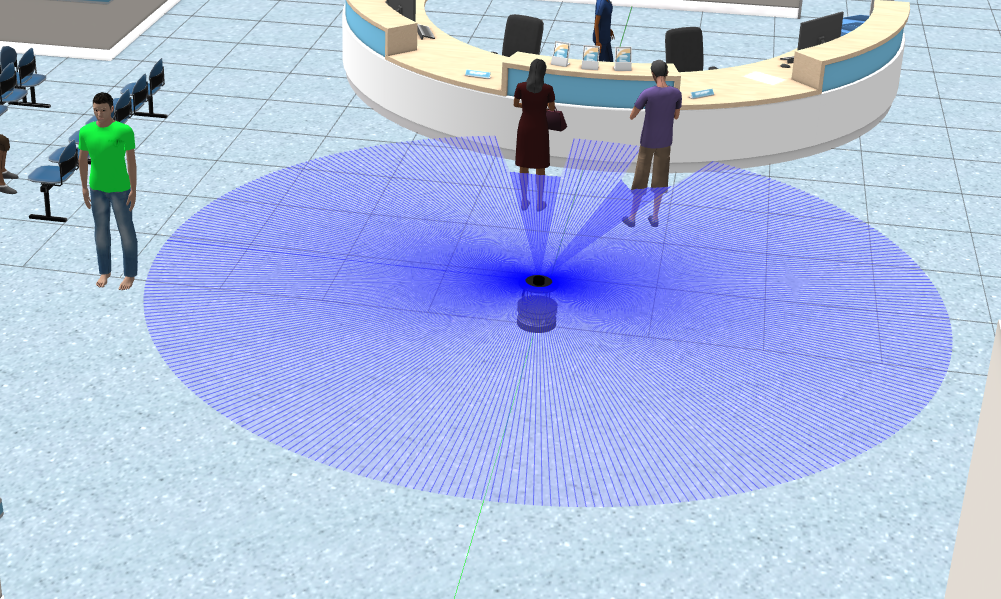
\includegraphics[width=7cm]{figs/c3/gazebo_sim.png}
    \end{center}
    \caption[Simulador Gazebo.]{Ejemplo de ejecución en gazebo.}
    \label{fig:gazebo_example}
\end{figure}

\subsection{TurtleBot2 simulado}
\label{subsec:turtlebot2_sim}
% ** TURTLEBOT2 -> SIMULADOR

Para algunas partes del proyecto, como el desarrollo de \textit{drivers} para ROS2 (\ref{cap:capitulo4}) o el comportamiento VFF usando
máquinas de estados (\ref{cap:capitulo6}), el simulador ha servido para probar y desarrollar los algoritmos. Para esto, se ha usado un modelo del
TurtleBot2 que cuenta con los mismos sensores (cámara, \textit{RPLIDAR}, \textit{bumper}, etc) que el real, así como los mismos \textit{topics}.

Este modelo del robot se obtiene del repositorio de
\textit{RoboticsInfrastructure}\footnote{\textbf{Robotics\_Infrastructure}: \url{
    https://github.com/JdeRobot/RoboticsInfrastructure/tree/humble-devel/CustomRobots/Turtlebot2/turtlebot2_simulated}},
donde podemos acceder los modelos \textit{URDF}\footnote{\textbf{URDF}: Unified Robot Description Format} tanto de la base
\textit{kobuki}\footnote{\textbf{kobuki\_description}:\url{
    https://github.com/JdeRobot/RoboticsInfrastructure/tree/humble\-devel/CustomRobots/Turtlebot2/turtlebot2_simulated/kobuki_description}}
como del cuerpo del Turtlebot2\footnote{\textbf{TurtleBot2}: \url{
    https://github.com/JdeRobot/RoboticsInfrastructure/tree/humble\-devel/CustomRobots/Turtlebot2/turtlebot2_simulated/turtlebot2}}
(incluyendo los sensores cámara y láser).

\begin{figure} [H]
    \begin{center}
        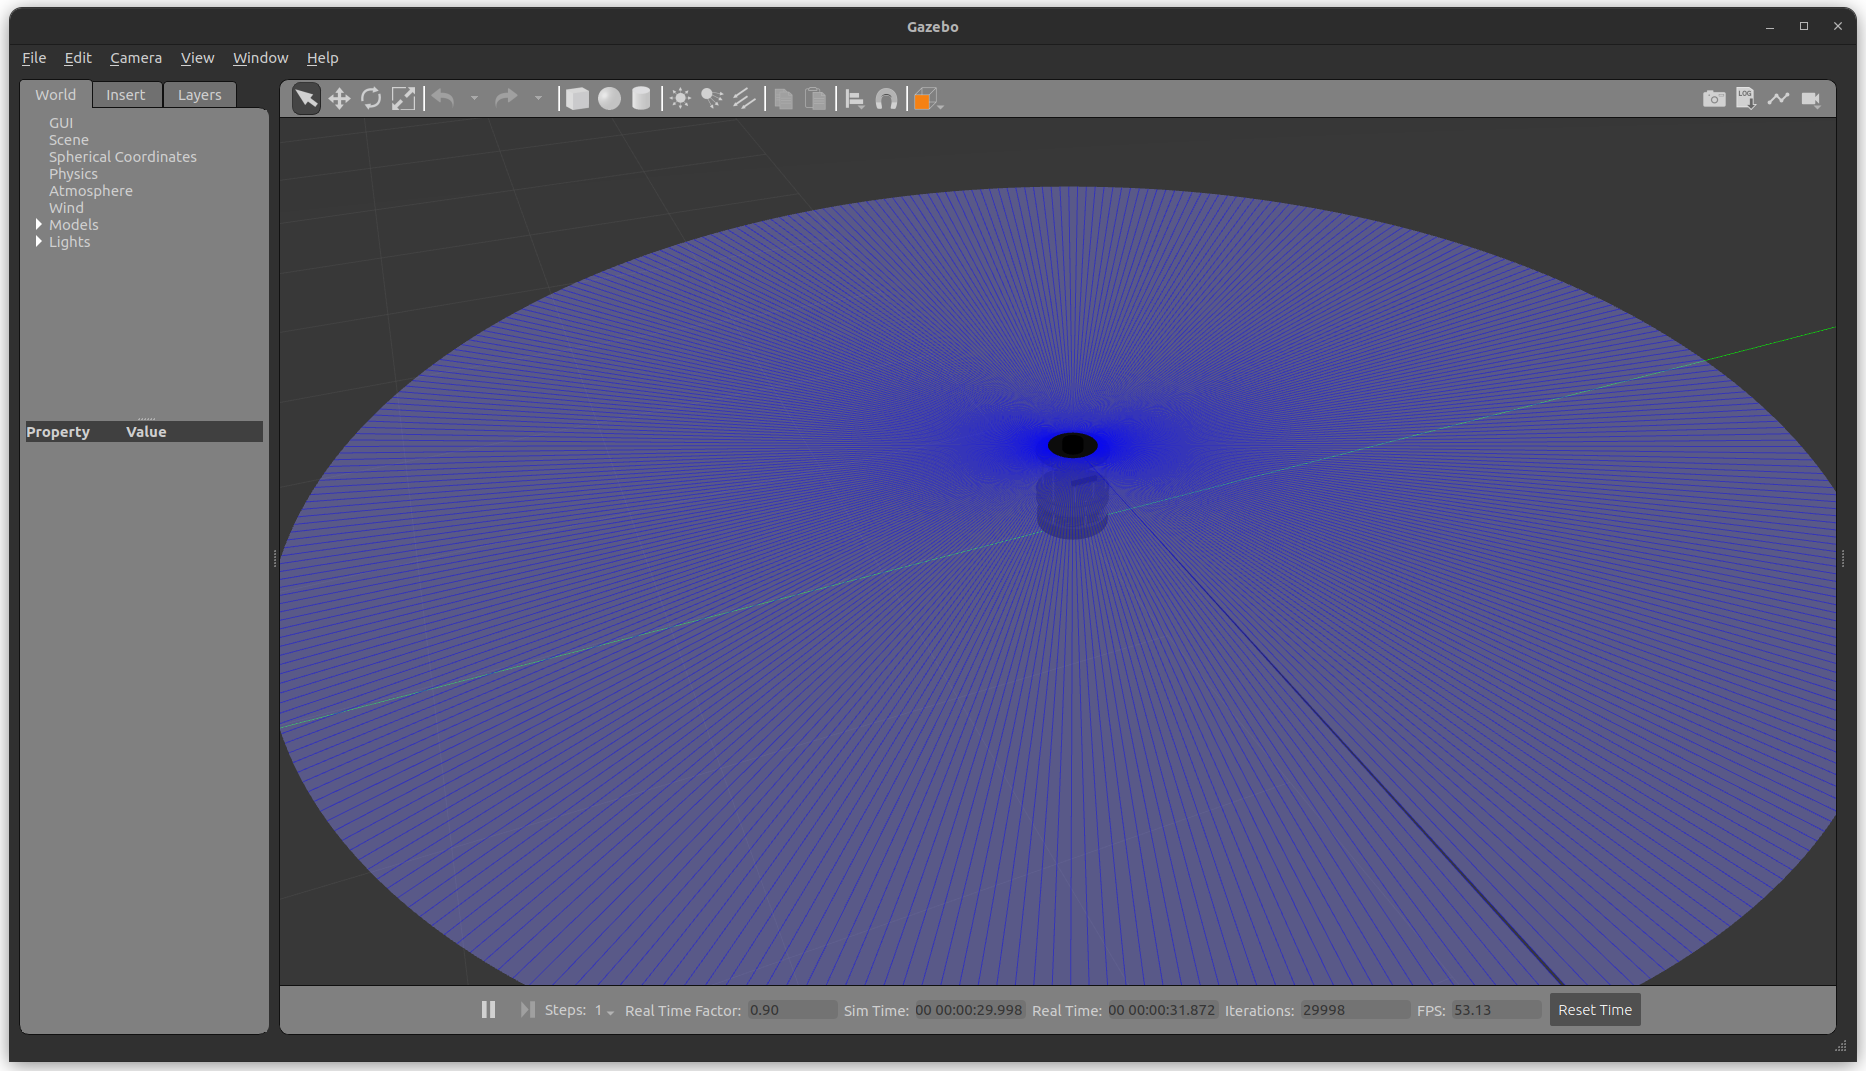
\includegraphics[width=14cm]{figs/c3/turtlebot2_sim.png}
    \end{center}
    \caption[TurtleBot2 simulado]{TurtleBot2 en gazebo.}
    \label{fig:turtlebot_2_sim}
\end{figure}
 

\section{VisualCircuit}
\label{sec:visualcircuit}
% ** VISUALCIRCUIT

VisualCircuit\footnote{\textbf{VisualCircuit Docs}: \url{https://jderobot.github.io/VisualCircuit/}} es un editor visual online basado en
programación por bloques de código orientado al desarrollo de aplicaciones robóticas. Está desarrollado sobre
IceStudio\footnote{\textbf{IceStudio Project}: \url{https://github.com/FPGAwars/icestudio}}.\\

\begin{figure} [H]
    \begin{center}
        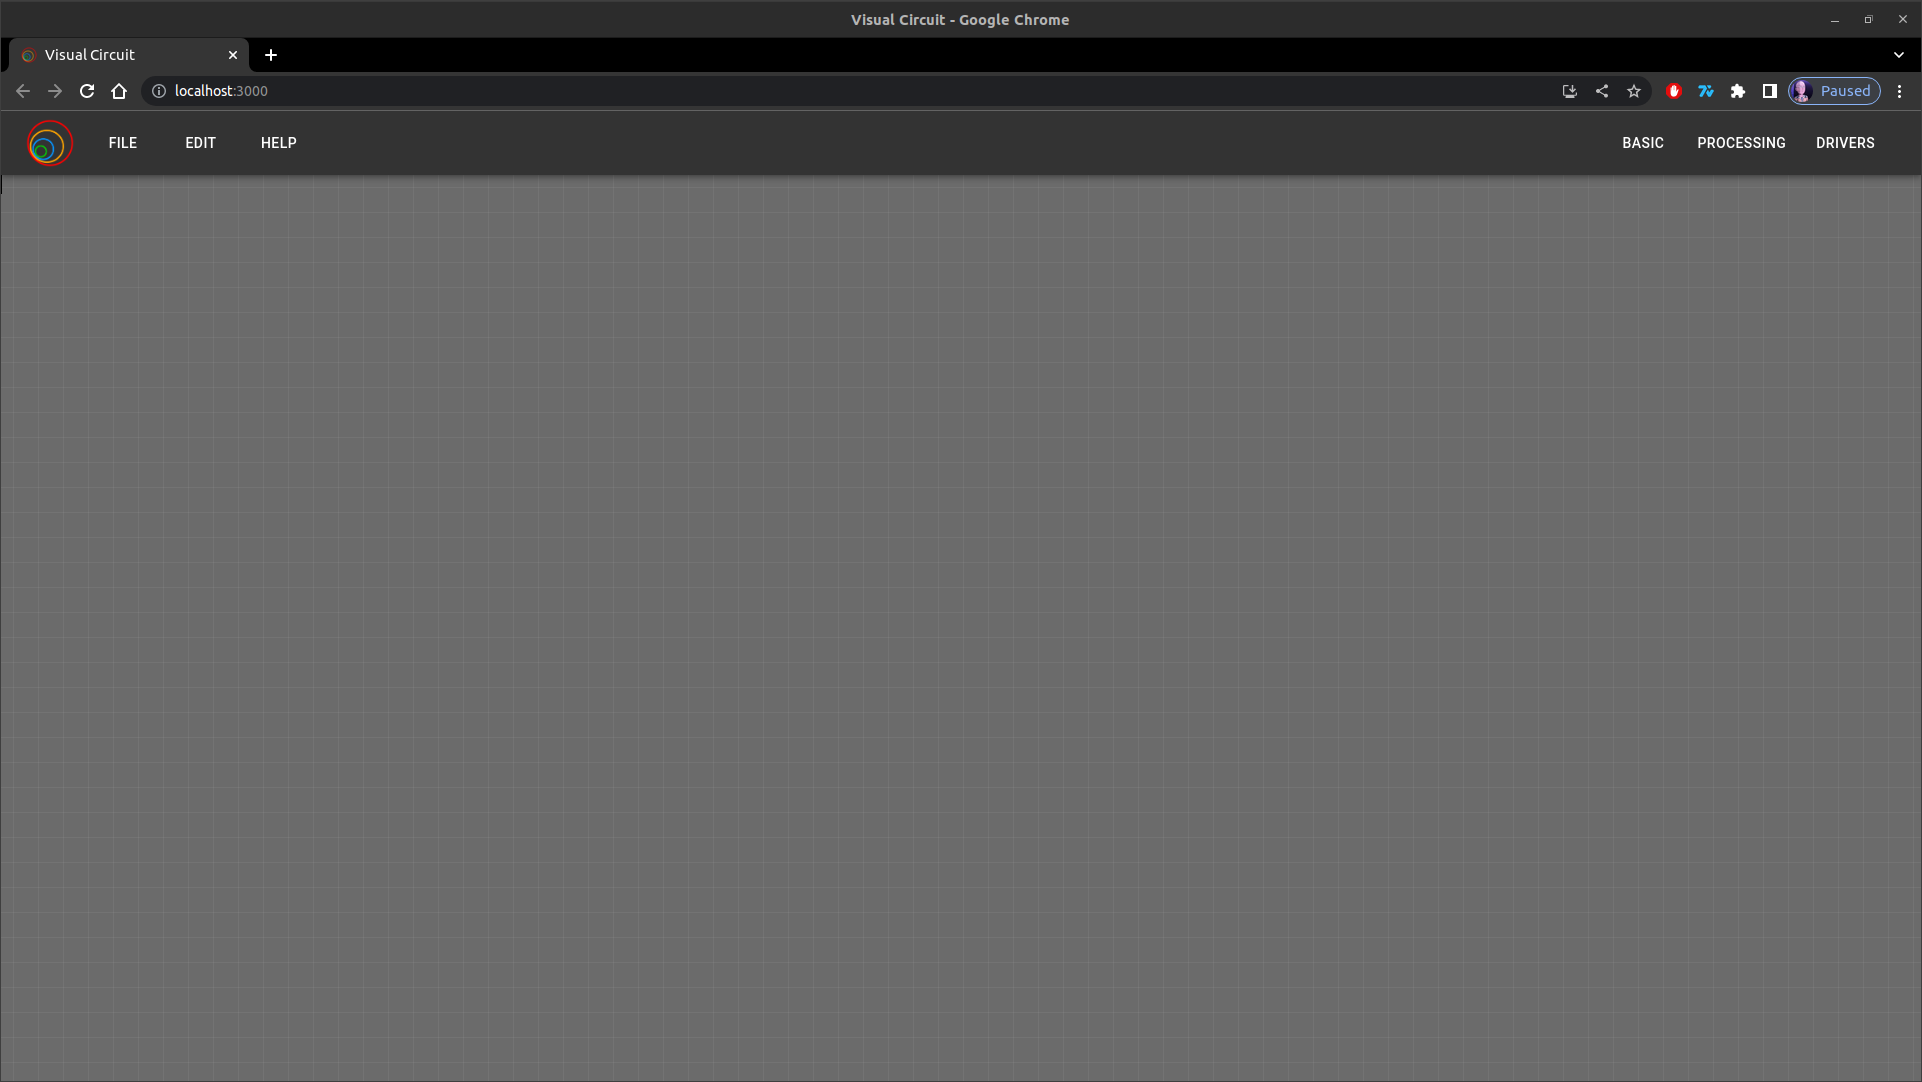
\includegraphics[width=13cm]{figs/c3/empty_VC.png}
    \end{center}
    \caption[VisualCircuit]{Página de VisualCircuit.}
    \label{fig:VC_empty}
\end{figure}

Los bloques que se pueden usar están divididos en varias pestañas: \textit{basics}, \textit{processing} y \textit{drivers}.
\begin{itemize}
    \item \textit{Basic:} bloques simples, como inputs y outputs, bloques para definir parámetros y constantes, o bloques para insertar código propio.
    \item \textit{Processing:}
    \begin{itemize}
        \item \textit{Control:} bloques de control (PID).
        \item \textit{OpenCV:} bloques relacionados con OpenCV\footnote{\textbf{OpenCV}: \url{https://opencv.org/}} y edición de imagen (filtros de color, detección de contornos, erosión, etc).
        \item \textit{TensorFlow:}un bloque para detección de objetos.
    \end{itemize}
    \item \textit{Drivers:} drivers que conectan con los sensores y actuadores
    \begin{itemize}
        \item \textit{Control:} motordriver (ROS) y teleoperador.
        \item \textit{OpenCV:} lector de imagenes desde archivos y desde cámaras, pantalla para mostrar las imágenes.
        \item \textit{ROS-Sensors:}  cámara, odometría e IMU\footnote{\textbf{IMU}: Inertial Measurement Unit} usando ROS.
    \end{itemize}
\end{itemize}

Para crear un bloque propio, se deben añadir varios bloques prefabricados. Para introducir el código principal se usa el bloque genérico,
como se puede ver en la figura \ref{fig:VC_creando_bloque}. Al crearlo, se permite definir el número de entradas, salidas y parámetros que tendrá el código.

\begin{figure} [H]
    \begin{center}
        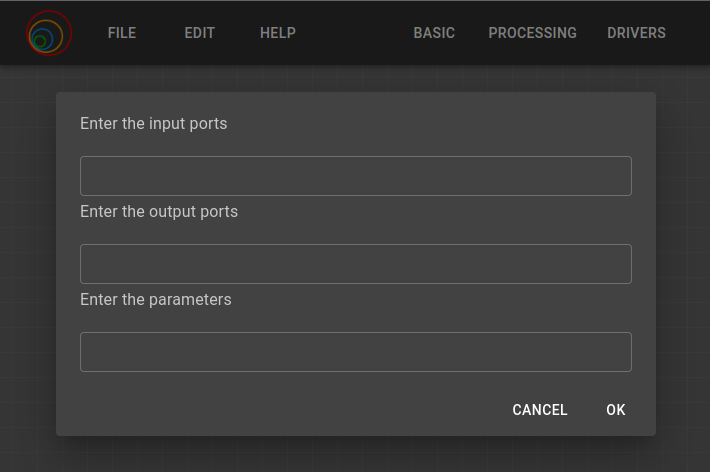
\includegraphics[width=9cm]{figs/c4/VC_pre_codeblock.png}
    \end{center}
    \caption[Creando un bloque en VisualCircuit]{Creando un bloque en VisualCircuit.}
    \label{fig:VC_creando_bloque}
\end{figure}

Una vez definidos, se deben usar bloques de \textit{Input}, \textit{Output} y \textit{Constant} y así, pulsando en ``\textit{Save as}'',
se exporta para usarlo como un bloque nuevo.
\begin{figure} [H]
  \begin{center}
      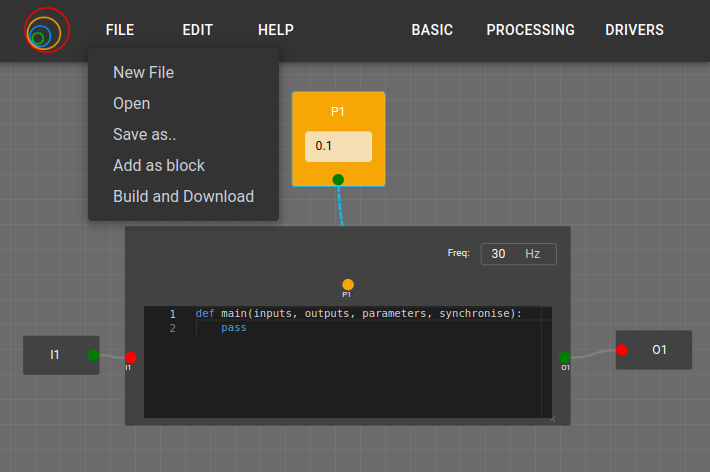
\includegraphics[width=10cm]{figs/c4/VC_saveas.png}
  \end{center}
  \caption[Guardando un bloque en VisualCircuit]{Guardando un bloque en VisualCircuit.}
  \label{fig:VC_saveas_bloque}
\end{figure}

Cuando se hayan generado varios bloques, se puede usar la opción \textit{FILE} \overrightarrow{ } \textit{Add as block} para añadirlos como nuevos bloques
y así formar un circuito completo con el comportamiento que se desee.
\begin{figure} [H]
  \begin{center}
      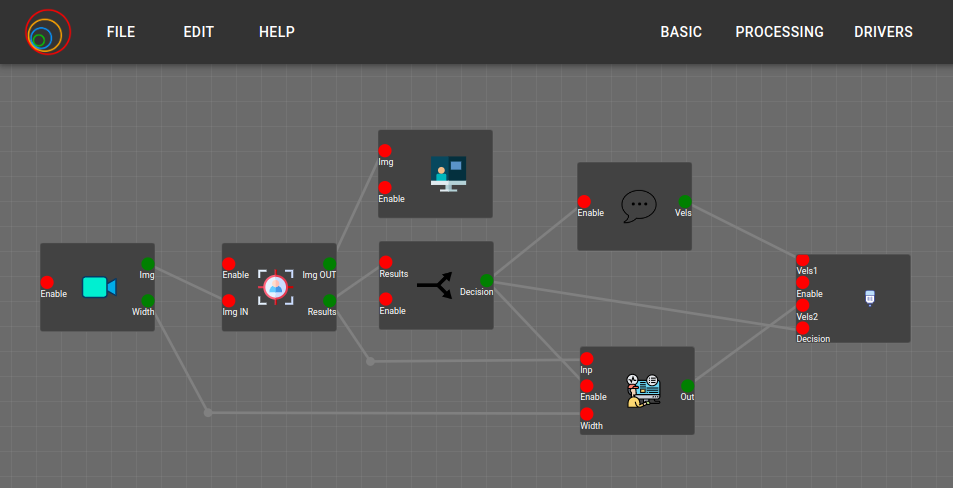
\includegraphics[width=10cm]{figs/c4/VC_example.png}
  \end{center}
  \caption[Ejemplo de proyecto en VisualCircuit]{Ejemplo de proyecto en VisualCircuit.}
  \label{fig:VC_example}
\end{figure}






